
\chapter{Simulation Time Delay Tele-operation}
\label{c7_DI_equimomental}
In this chapter simulation of a teleoperated mobile platform is presented. In tele-operation the human operators observe a remote scene through camera/s, and manipulating the local steering wheel and accelerator paddle as shown in figure \ref{fig:teleoperation} . The command is transmitted to the mobile robot over wireless network. The operator response is based on the latest feedback images from the cameras. In general there is time lag when communication take place over wireless network. The time lag deteriorates the human performance as discussed in \cite{chen2007human} and references there in.  The this chapter simulation of teleoperation both for delayless and delay transmission network are presented.
\begin{figure}
	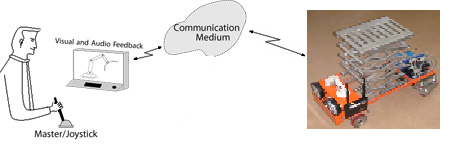
\includegraphics[width=\linewidth,keepaspectratio]{Chapter6/fig/teleoperation}
	\captionof{figure}{Teleoperation  Architecture }
	\label{fig:teleoperation} 
\end{figure}

\section{Modeling of mobile platform}
The standard kinematic model as described in \cite{campion1996structural} of the mobile platform is used for the simulation. This use of kinematic is justified as  the vehicle is expected to move at relatively slow speed and model is simple. Inputs to the model are left and right rear wheel velocities. The front wheels are steered to satisfy the Ackerman condition as presented in **** and are assumed to attain the desired angle instantaneously. Therefore the robot can be treated as differential drive robot.  The kinematic model of the platform is presented below

\begin{equation}
\begin{pmatrix}
\dot{x}\\ 
\dot{y}\\ 
\dot{\theta}
\end{pmatrix}
=
\begin{pmatrix}
\cos \theta & 0 \\
\sin \theta & 0 \\
0& 1
\end{pmatrix}
\begin{pmatrix}
r_w/2 & r_w/2\\
1/b & -1/b
\end{pmatrix}
\begin{pmatrix}
\dot{\phi_L}\\
\dot{\phi_R}
\end{pmatrix}
\end{equation}


Where ,  $b$ is the distance between the rear wheels, $r_w$ wheel radius. $\dot{\phi_R}$ and $\dot{\phi_L} $ are the left and right wheel rotational velocity. 

The operator station sends the command $u_1$ and $u_2$ over the wireless network, in general it will be delayed by $\delta$ time. These commands are interpreted by the robot controller as the left and right wheel velocities.  Therefore by taking the time delay into consideration we can write
\begin{equation}
\begin{pmatrix}
\dot{\phi_R}(t) \\
 \dot{\phi_L}(t)
\end{pmatrix}
=
\begin{pmatrix}
u_r(t-\delta)\\
u_1(t-\delta)
\end{pmatrix}
\end{equation}

The control inputs to the mobile robot  $u_1$ and $u_2$ are generate by the operator based on the visual data available to him. We next present the model of the human operator to be used for simulation the complete loop.


\section{Modeling the human operator}
In order to simulate the teleoperation loop we need a mathematical model of human operator. The mathematical  modelling of the operator`s action is modelled assuming a car driving metaphor. The video feedback, which the he receives of the remote environment, give him the idea of the vehicles  position and the tentative next goal point (p) based on a lookahead distance (l). He then constructs a  virtual path mentally and tries to manoeuvre or steers the robot to follow that path as shown in figure \ref{fig:drivingStratagy}. As he moves forward the goal point keeps changing until he reaches the desired location. This methodology of path tracing is known as pure pursuit \cite{coulter1992implementation} or following the carrot strategy. 
\begin{figure}
	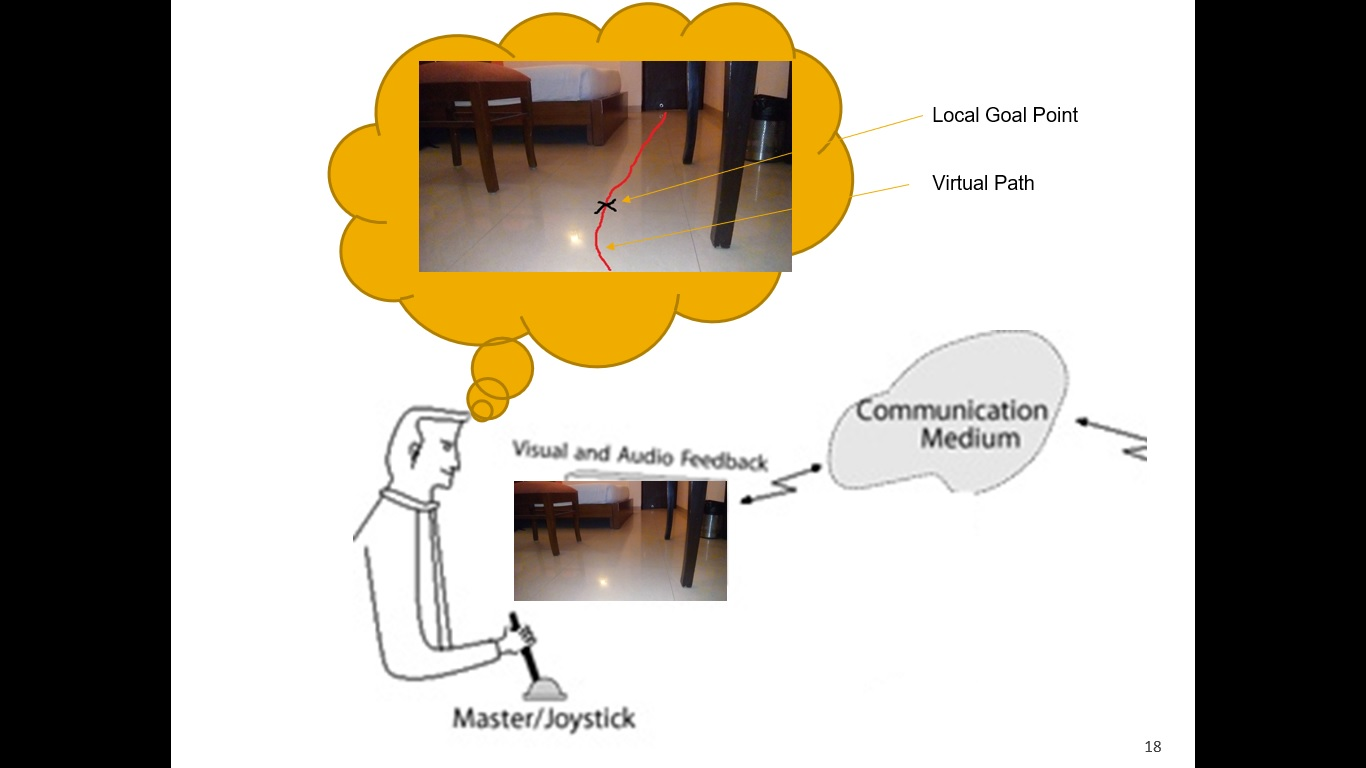
\includegraphics[width=\linewidth,keepaspectratio]{Chapter6/fig/mentalMap}
	\captionof{figure}{Assumed driving strategy  }
	\label{fig:drivingStratagy} 
\end{figure}

The mathematical model for the pure pursuit method of path following can be derived as given in figure \ref{fig:purePGeo}.
As shown in figure \ref{fig:purePGeo}, the origin of the coordinate system is at point $o$, the middle of rear axis of the robot. Since the differential drive robot  can move only about a circle with center  lying on the line along its rear axis, a arc $op$ of radius $r$, is drawn with center $o1$ and passing through $o$ and $p$. Where $p$ is a point on the path to be traced by the robot. The linear distance $l$ between the points $o$ and  $p$ is called the look ahead distance. This distance in the case of a teleoperated robot will depend on the field of view of the remote location camera and the obstacles in present in the remote environment.

If $(x,y)$ is the coordinate of point $p$ in $X-Y$ coordinate system, then 
\begin{equation}
x^2+y^2=l^2, \quad \quad d=r-x
\end{equation}

Similarly, from triangle $p, x, o1$ we get
\begin{equation}
d^2+y^2=r^2\quad \Rightarrow (r-x)^2+y^2=r^2 \quad \Rightarrow x^2+y^2-2rx=0
\end{equation}
Replacing $x^2$ and $y^2$ in equation 6.4 with 6.3 we get
\begin{equation}
2rx=l^2\quad \quad \Rightarrow r=\frac{l^2}{2x}
\end{equation}
\begin{figure}
	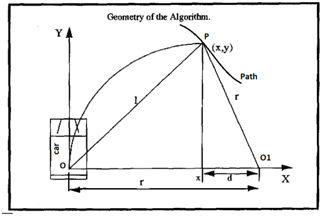
\includegraphics[width=\linewidth,keepaspectratio]{Chapter6/fig/purepesuitgeometry}
	\captionof{figure}{Geometry of Pure Pursuit }
	\label{fig:purePGeo} 
\end{figure}

Once, the radius $r$ the desired  linear velocity $v$ of robot is known the angular velocity of the vehicle is $\dot{\theta}=-v/r$. The rear wheel desired velocities $\dot{\phi_d(t)}$ and $\dot{\phi_(t)}$ can be calculated from equation 6.1. Where $\dot{y}=v$ and to match the orientation of vehicle with that in  figure \ref{fig:purePGeo} we set $\theta=90^o$. We get

\begin{equation}
\begin{pmatrix}
\dot{x}\\
\dot{y}\\
\dot{\theta}
\end{pmatrix}
=
\begin{pmatrix}
0 & 0 \\
r_w/2 & r_w/2 \\
b/2 & -b/2
\end{pmatrix}
\begin{pmatrix}
\dot{\phi_L}\\
\dot{\phi_R}
\end{pmatrix}
\quad \Rightarrow 
\begin{pmatrix}
\dot{\phi_L}\\
\dot{\phi_R}
\end{pmatrix} =
\begin{pmatrix}
1/r_w/ & 1/r_w \\
1/b & -1/b
\end{pmatrix}
\begin{pmatrix}
v\\
\dot{\theta}
\end{pmatrix}
\end{equation}
This is the signal which the operator sends over the  communication network to the robot as command at time $t$. Therefore
\begin{equation}
\begin{pmatrix}
u_r(t)\\
u_1(t)
\end{pmatrix}
=
\begin{pmatrix}
1/r_w/ & 1/r_w \\
1/b & -1/b
\end{pmatrix}
\begin{pmatrix}
v\\
\dot{\theta}
\end{pmatrix}
\end{equation}  
\section{Teleoperation loop}
\section{Simulation Results }
\section{Predictive Model based Feedback}
\subsection{Using Dynamic model of vehicle}
\subsection{Kalman Filter with odometer data and Accelorometer?}


\section{Summary}
In this chapter, 